\documentclass{article}

\usepackage{fullpage}
\usepackage{url}
\usepackage{graphicx}
\usepackage{amsmath}
\usepackage{physics}
\usepackage{mathtools}
\usepackage{bbold}

\DeclareMathOperator{\erfi}{erfi}
\newcommand{\R}{\ensuremath{\mathbb{R}}}
\newcommand{\C}{\ensuremath{\mathbb{C}}}
\newcommand{\Z}{\ensuremath{\mathbb{Z}}}

\title{Statistical Mechanics I Test}
\author{Idan Stark}
\date{\today}

\begin{document}
\maketitle

\section{A microscopic model with two $\Z_2$ symmetries}
In this section we consider a lattice model with two Ising spins on each site $i$:
\begin{equation}
    \sigma_i =\pm1 \qquad \tau_i = \pm1
\end{equation}
With the Hamiltonian:
\begin{eqnarray}
    \beta H = -J_\sigma \sum_{\langle i, j \rangle}\sigma_i \sigma_j -J_\tau \sum_{\langle i, j \rangle}\tau_i \tau_j - K \sum_{\langle i, j \rangle}(\sigma_i \sigma_j)(\tau_i \tau_j)
\end{eqnarray}
Defined over a regular lattice with coordinate number $z$ and no external fields. This means that Hamiltonian is invariant under two independent gloabl $\Z_2$ symmetries:
\begin{equation}
    \left\{\sigma_i\right\} \rightarrow -\left\{\sigma_i\right\}
    \qquad
    \left\{\tau_i\right\} \rightarrow -\left\{\tau_i\right\}
\end{equation}
Let us define the uniform order parameters:
\begin{equation}
    m_\sigma = \langle \sigma_i \rangle
    \qquad
    m_\tau = \langle \tau_i \rangle
\end{equation}
\subsection{Uniform mean-field decoupling}
To use the mean field approximation for this model, let us approximate each bond:
\begin{equation}
    \sigma_i \sigma_j \approx \sigma_i m_\sigma + \sigma_j m_\sigma - m_\sigma^2
    \qquad
    \tau_i \tau_j \approx \tau_i m_\tau + \tau_j m_\tau - m_\tau^2
\end{equation}
and decouple the interaction:
\begin{equation}
\begin{gathered}
    (\sigma_i \sigma_j) (\tau_i \tau_j) \approx (\sigma_i \sigma_j)m_\tau^2 + (\tau_i\tau_j)m_\sigma^2 - m_\sigma^2m_\tau^2 \approx \\ \approx
    (\sigma_i m_\sigma + \sigma_j m_\sigma - m_\sigma^2)m_\tau^2 + (\tau_i m_\tau + \tau_j m_\tau - m_\tau^2)m_\sigma^2 - m_\sigma^2m_\tau^2 = \\ =
    m_\tau^2m_\sigma(\sigma_i + \sigma_j) +
    m_\sigma^2m_\tau(\tau_i + \tau_j) - 3m_\sigma^2m_\tau^2
\end{gathered}
\end{equation}
Plugging this into the Hamiltonian gives:
\begin{equation}
\begin{gathered}
    \beta H = \sum_{\langle i, j \rangle}\left[
        -J_\sigma(\sigma_i m_\sigma + \sigma_j m_\sigma - m_\sigma^2)
        -J_\tau(\tau_i m_\tau + \tau_j m_\tau - m_\tau^2)
        -K(m_\tau^2m_\sigma(\sigma_i + \sigma_j) + m_\sigma^2m_\tau(\tau_i + \tau_j) - 3m_\sigma^2m_\tau^2)
    \right] = \\ =
    \sum_{\langle i, j \rangle}\left[
        -(J_\sigma m_\sigma + K m_\tau^2m_\sigma)(\sigma_i + \sigma_j)
        -(J_\tau m_\tau + K m_\sigma^2m_\tau)(\tau_i + \tau_j)
        + J_\sigma m_\sigma^2
        + J_\tau m_\tau^2
        + 3Km_\sigma^2m_\tau^2
    \right]
\end{gathered}
\end{equation}
The sum has no interactions between $(\sigma_i, \tau_i)$ and $(\sigma_j, \tau_j)$, and therefore can be rewritten as a sum over the spins instead of nearest neighbors bonds. Since each spin has $z$ bonds, it appears in $z$ terms of the above sum. The number of bonds is just half the number of spins. This gives:
\begin{equation}
\begin{gathered}
    \beta H = \sum_i \left[
        -z(J_\sigma m_\sigma + K m_\tau^2m_\sigma)\sigma_i
        -z(J_\tau m_\tau + K m_\sigma^2m_\tau)\tau_i
        + \frac{z}{2}J_\sigma m_\sigma^2
        + \frac{z}{2}J_\tau m_\tau^2
        + 3\frac{z}{2}Km_\sigma^2m_\tau^2
    \right] = \\ =
    \sum_i \left[
        -z(J_\sigma m_\sigma + K m_\tau^2m_\sigma)\sigma_i
        -z(J_\tau m_\tau + K m_\sigma^2m_\tau)\tau_i
    \right]
    + N\frac{z}{2}\left(J_\sigma m_\sigma^2
    + J_\tau m_\tau^2
    + 3Km_\sigma^2m_\tau^2\right)
\end{gathered}
\end{equation}
Which can be rewritten as:
\begin{equation}
    \beta H = \sum_i \left[-h_\sigma \sigma_i - h_\tau \tau_i\right] + N\beta f_0(m_\sigma, m_\tau)
\end{equation}
Where we defined:
\begin{equation}
    h_\sigma = z(J_\sigma m_\sigma + K m_\tau^2m_\sigma)
    \qquad
    h_\tau = z(J_\tau m_\tau + K m_\sigma^2m_\tau)
    \qquad
    \beta f_0 = \frac{z}{2}\left(
        J_\sigma m_\sigma^2 + J_\tau m_\tau^2 + 3Km_\sigma^2m_\tau^2
    \right)
\end{equation}
Let us now write the partition function $Z$ in terms of $m_\sigma$ and $m_\tau$:
\begin{equation}
\label{eq:partition1}
\begin{gathered}
    Z = \sum_{\sigma_1=\pm1}\sum_{\tau_1=\pm1}\cdots\sum_{\sigma_N=\pm1}\sum_{\tau_N=\pm1}e^{\sum_i \left[-h_\sigma \sigma_i - h_\tau \tau_i\right] + N\beta f_0(m_\sigma, m_\tau)} = \\ =
    e^{N\beta f_0(m_\sigma, m_\tau)}\sum_{\sigma_1=\pm1}\sum_{\tau_1=\pm1}\cdots\sum_{\sigma_N=\pm1}\sum_{\tau_N=\pm1}\prod_i e^{-h_\sigma \sigma_i}e^{- h_\tau \tau_i}
\end{gathered}
\end{equation}
Each site gives:
\begin{equation}
    \sum_{\sigma_i=\pm1}\sum_{\tau_i=\pm1} e^{-h_\sigma \sigma_i}e^{- h_\tau \tau_i} = e^{h_\sigma + h_\tau} + e^{-h_\sigma - h_\tau} + e^{-h_\sigma + h_\tau} + e^{-h_\sigma + h_\tau} = 4\cosh(h_\sigma)\cosh(h_\tau)
\end{equation}
Therefore:
\begin{equation}
\label{eq:partition2}
    Z = e^{N\beta f_0(m_\sigma, m_\tau)}4^N\left[\cosh(h_\sigma)\cosh(h_\tau)\right]^N
\end{equation}
From the original partition function in equation \ref{eq:partition1}, we can see that $m_\sigma$ and $m_\tau$ follow the formula for magnetization:
\begin{equation}
    m_\sigma = \langle \sigma_i \rangle = \frac{1}{N}\sum_i \sigma_i = \frac{1}{N}\frac{\partial \ln Z}{\partial h_\sigma}
    \qquad
    m_\tau = \langle \tau_i \rangle = \frac{1}{N}\sum_i \tau_i = \frac{1}{N}\frac{\partial \ln Z}{\partial h_\tau}
\end{equation}
Plugging $Z$ from equation \ref{eq:partition2} into it gives the self-consistency equations:
\begin{equation}
\begin{cases}
    m_\sigma = \tanh(z(J_\sigma + K m_\tau^2)m_\sigma)
    \\
    m_\tau = \tanh(z(J_\tau + K m_\sigma^2)m_\tau)
\end{cases}
\end{equation}
\subsection{Linear stability and critical lines}
Let us now linearize the equations near the paramagnet $m_\sigma = m_\tau = 0$ using $\tanh(x) \approx x$:
\begin{equation}
\begin{cases}
    m_\sigma = z(J_\sigma + K m_\tau^2)m_\sigma
    \\
    m_\tau = z(J_\tau + K m_\sigma^2)m_\tau
\end{cases}
\end{equation}
Assuming $m_\sigma, m_\tau \ne 0$, we can divide by $m_\sigma$ and $m_\tau$ respectively:
\begin{equation}
\begin{cases}
    1 = zJ_\sigma + zK m_\tau^2
    \\
    1 = zJ_\tau + zK m_\sigma^2
\end{cases}
\end{equation}
And solving for $m_\sigma$ and $m_\tau$:
\begin{equation}
    m_\sigma = \pm \sqrt{\frac{1 - zJ_\sigma}{zK}}
    \qquad
    m_\tau = \pm \sqrt{\frac{1 - zJ_\tau}{zK}}
\end{equation}
We got three options for each order parameter: these two roots and 0. For the roots to exist, we assumed $zJ_i < 1$ for $i = \sigma, \tau$. Therefore, when $zJ_i > 1$, that order parameter has only one solution at $m_i = 0$. In other words, the condition for the onset of ordering for each order parameter $m_i$ is $zJ_i < 1$.
\newline
The critical lines $zJ_i = 1$ define the phase transformation, which are unaffected by the interaction term $K$ up to the linear order. This is a result of the linearization of the self consistency equations: the interaction term is only related to higher order effects on the critical lines via higher order derivatives of $\tanh$.
\subsection{Landau expansion and "copmetition vs cooperation"}
The free energy density is just the free energy divided by $N$:
\begin{equation}
    f_{MF} = \beta f_0(m_\sigma, m_\tau) + \ln(4) + \ln\cosh(h_\sigma) + \ln\cosh(h_\tau)
\end{equation}
Using the approximation:
\begin{equation}
    \ln\cosh(x) = \frac{1}{2}x^2 - \frac{1}{12}x^4 + \cdots
\end{equation}
We can write the free energy density that as a polynomial in $m_\sigma$ and $m_\tau$ gives:
\begin{equation}
\begin{gathered}
    f_{MF} \approx \beta zJ_\sigma m_\sigma^2 + \beta zJ_\tau m_\tau^2 + 3\beta zKm_\sigma^2 m_\tau^2 + \ln(4) + \left(\frac{h_\sigma^2 + h_\tau^2}{2} - \frac{h_\sigma^4 + h_\tau^4}{12}\right) = \\ =
    \ln4 +
    \left(\beta zJ_\sigma + \frac{1}{2}z^2J_\sigma^2\right)m_\sigma^2 +
    \left(\beta zJ_\tau + \frac{1}{2} z^2J_\tau^2\right)m_\tau^2 +
    \left(-\frac{1}{12}z^2J_\sigma^4\right)m_\sigma^4 + \\ +
    \left(-\frac{1}{12}z^2J_\tau^4\right)m_\tau^4 +
    \left(3\beta zK + J_\sigma K + J_\tau K\right)m_\sigma^2m_\tau^2 +
    O(m^6)
\end{gathered}
\end{equation}
Renaming:
\begin{equation}
\begin{gathered}
    r_\sigma = 2\beta zJ_\sigma + z^2J_\sigma^2
    \qquad
    u_\sigma = -\frac{1}{3}z^2J_\sigma^4
    \\
    r_\tau = 2\beta zJ_\tau + z^2J_\tau^2
    \qquad
    u_\tau = -\frac{1}{3}z^2J_\tau^4
    \\
    v = 6\beta zK + 2J_\sigma K + 2J_\tau K
\end{gathered}
\end{equation}
Gives:
\begin{equation}
    f_{MF} = k_BT\ln4 + \frac{r_\sigma}{2}m_\sigma^2 + \frac{r_\tau}{2}m_\tau^2 + \frac{u_\sigma}{2}m_\sigma^4 + \frac{u_\tau}{2}m_\tau^4 + \frac{v}{2}m_\sigma^2m_\tau^2 + O(m^6)
\end{equation}
Let us now focus on $v$. It can be writeten as:
\begin{equation}
    v = 2(3\beta z + J_\sigma + J_\tau) K
\end{equation}
Since $\beta, z, J_\sigma, J_\tau$ are positive (for ferromagnetic models), the interaction $v$ has the same sign as $K$.

\section{Landau theory with two $\Z_2$ symmetries}
Let us now consider the matching Landau theory, with two scalar order parameters $\phi_1$ and $\phi_2$ with the independent $\Z_2$ symmetries:
\begin{equation}
    \phi_1 \rightarrow -\phi_1
    \qquad
    \phi_2 \rightarrow -\phi_2
\end{equation}
and no external fields. The most general form of the Landau free energy density is then:
\begin{equation}
    F = const +
    \frac{r_1}{2}\phi_1^2 +
    \frac{r_2}{2}\phi_2^2 +
    \frac{u_1}{4}\phi_1^4 +
    \frac{u_2}{4}\phi_2^4 +
    \frac{v}{2}\phi_1^2\phi_2^2 +
    O(m^6)
\end{equation}
\subsection{The most general landau free energy}
The theory must be bounded from below along every line in the $(\phi_1, \phi_2)$ plain.
\newline
Along the $\phi_1 = 0$ line, the theory acts like an Ising theory and therefore $u_2$ must be positive. $u_1 > 0$ for the same reason. There are no conditions on $r_1$ and $r_2$.
\newline
Let us now look at $v$. Along every straight line passing throguh the origin $\phi_2 = a \phi_1 \equiv \phi$, the model is reduced to the Ising model:
\begin{equation}
    F = const +
    \frac{r_1 + ar_2}{2}\phi^2 +
    \frac{u_1 + a^4u_2 + 2a^2v}{4}\phi^4 +
    O(m^6)
\end{equation}
So, along this line:
\begin{equation}
    u_1 + a^4u_2 + 2a^2v > 0
\end{equation}
This must be true for every $a$, therefore. Since $u_2 > 0$, this is satisfied if the polynomial has no roots:
\begin{equation}
    v^2 < u_1u_2
\end{equation}
\begin{equation}
    |v| < \sqrt{u_1u_2}
\end{equation}
In the edge case where the polynom has a single root, this classifies a single direction in which the system is constant. This is allowed because even though the free energy has no minima in that direction, it is constant and thus still bounded from below. So the condition is actually:
\begin{equation}
    |v| \le \sqrt{u_1u_2}
\end{equation}
The final caviate is that if $r_2 = 0$ and $v = 0$ we can allow $u_2 = 0$ as well, and then the model is reduced to a single Ising model in the $\phi_1$ direction. Similarly, if $r_1 = v = 0$ then we allow $u_1 = 0$. This is again allowed, since a constant function is still bounded from below.
\subsection{Phases and Minima}
Let us now look for the possible phases. The clear first phase is when both fields are zero. This is the paramagnetic phase, and it is always a local minimum.
\newline
The next phase is when one of the fields is zero, and the other is not. In that case, the non-zero field acts like an Ising field, and this phase will exist (i.e. the non-zero field will actually be $\ne 0$) if it's in the ordered stage.
In other words, the $\phi_1$-only phase exists as a local minima if $r_1 < 0$, while the $\phi_2$-only phase exists if $r_2 < 0$. If both $r_1 < 0$ and $r_2 < 0$, we get a phase where both fields can be non-zero, which is the coexistance phase.
\newline
However, this is only strictly true for $v = 0$. For $v \ne 0$, we get an interaction that shifts the magnetization of each of them. In other words, if for $v = 0, r_1 < 0, r_2 < 0$ the fields have minima at
\begin{equation}
    (\phi_1, \phi_2) = \left(
        \pm \sqrt{\frac{-r_1}{2u_1}},
        \pm \sqrt{\frac{-r_2}{2u_2}}
    \right)
\end{equation}
then the interaction term moves the minima point by changing the effective polynomial for each field\footnote{The calculation of the minima is not long but it was not part of the quesiton}.
\subsection{Phase diagram in a 2D slice}
Let us now look at the phase diagram over the $r_1, r_2$ plain for $u_1 = u_2 = 1$, at different values of $v$. Since $|v| < \sqrt{u_1u_2} = 1$, the important cases are (i) $v = 0$, (ii) $-1 < v < 0$, (iii) $0 < v < 1$, (iv) $v = -1$, and (v) $v = 1$.
\newline
Starting again from $v = 0$, this is the clear case of two coexsisting Ising models. For each of the fields $\phi_i: i=1,2$, if $r_i > 0$ the field is disordered, $\phi_i = 0$, and if $r_i < 0$ the field is ordered $\phi_i^2 = -\frac{1}{2}r_i$. The phase diagram can be seen in figure 1.
\begin{figure}[h]
    \label{fig:zero_v}
    \centering
    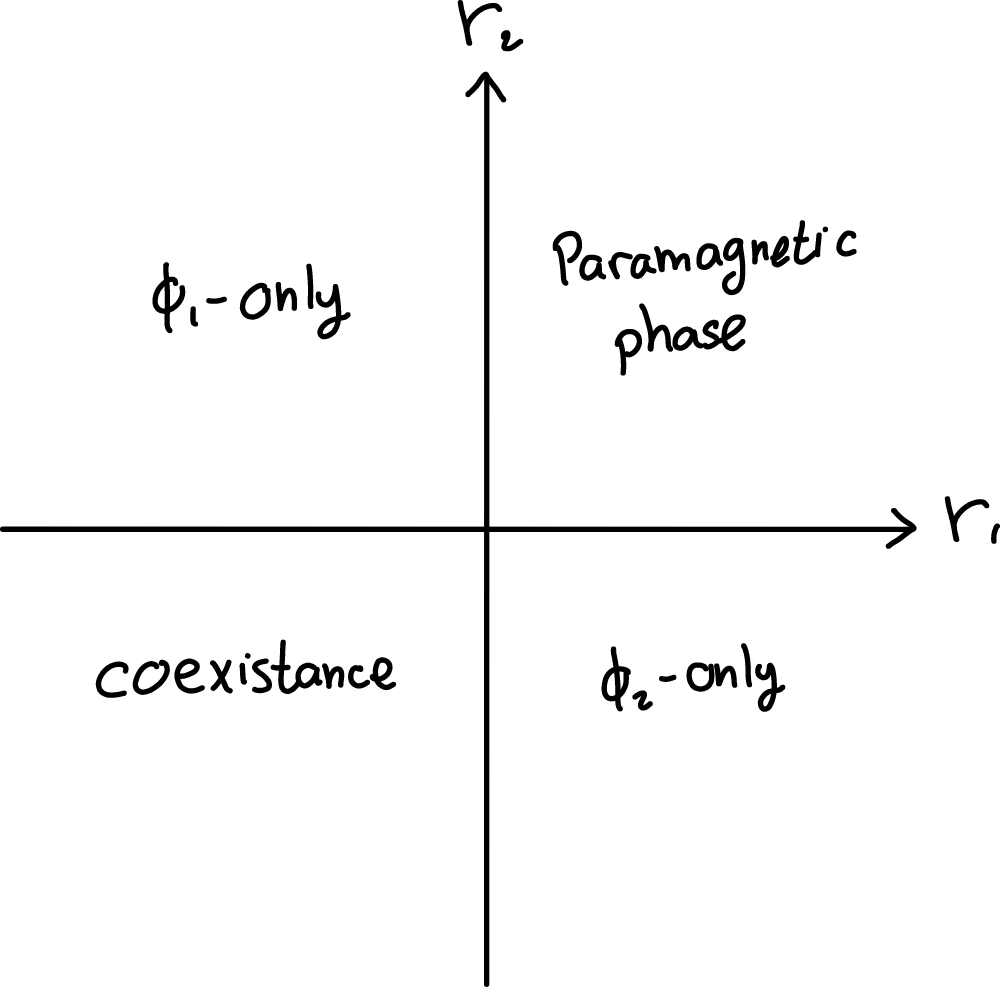
\includegraphics[width=0.5\textwidth]{Notewise-Untitled 2025-12-30-20260209195742.png}
    \caption{The phase diagram for $v = 0$}
\end{figure}
\newline
Let us now look at $v \ne 0, \pm 1$, and for convinence let us look at $\phi_1$, and merge the identical treatment of $\phi_2$ afterwards. For a given $\phi_2$, $\phi_1$ acts exactly as it would have with $v = 0$, except that now its qudaratic prefactor is $a_1 = \frac{1}{2}\left(r_1 + v\phi_2^2\right)$ instead of simply $\frac{1}{2}r_1$. In this case as well, for the free energy to have non zero minima, it is required that $a_1 < 0$. This can be analysed then in three cases. If $v > 0$ and $r_1 > 0$, then $a_1 > 0$ and $\phi_1$ is in its disordered phase $\phi_1 = 0$. If $r_1 < 0$ and $v < 0$ then $\phi_1$ is in its ordered phase $\phi_1^2 = -(r_1 + v\phi_2^2)$ (there is a dependency between the valeus of the fields here, we will get back to that when we cross this analysis with the same one for the other field).
\newline
In the third case, $v$ and $r_1$ have different signs. In this case, it's easy to solve the requirement $a_1 > 0$ to get:
\begin{equation}
\begin{cases}
    \phi_2^2 > -\frac{r_1}{v} : v > 0, r_1 < 0
    \\
    \phi_2^2 < -\frac{r_1}{v} : v < 0, r_1 > 0    
\end{cases}
\end{equation}
In the first case $v > 0$, for $\phi_1$ to have disordered phase, it requires $\phi^2$ to also be in a disordere phase (since it must be non-zero). This is not the case for $v < 0$, where $\phi_2 = $ is a solution to the above condition. This means that while for $v < 0$ there can be a $\phi_1$-only phase, for $v > 0$ there can only be a coexistance phase or a paramagnetic phase.
\newline
Let us merge this analysis with the matching analysis of the other field, starting from the $v < 0$ case, moving quadrant by quadrant in the $r_1,r_2$ plain.
\newline
If both $r_1 < 0$ and $r_2 < 0$, both fields are in their ordered phase, and we get a coexistance. Their values in this case can be found by solving:
\begin{equation}
\begin{cases}
    \phi_1^2 = -(r_1 + v\phi_2^2)
    \\
    \phi_2^2 = -(r_2 + v\phi_1^2)
\end{cases}
\end{equation}
To get:
\begin{equation}
\begin{cases}
    (\phi_1^2)_{min} = \frac{vr_2 - r_1}{1-v^2}
    \\
    (\phi_2^2)_{min} = \frac{vr_1 - r_2}{1-v^2}
\end{cases}
\end{equation}
Let us look now at the case where one of them is positive. Choosing without limitation of generality $r_1 > 0$ and $r_2 < 0$, then $\phi_1$ can be either ordered or disordered, based on the value of $\phi_2^2$.
Let us compare then the value of $\phi_2^2$ we found with the condition for $a_1 > 0$:
\begin{equation}
    \frac{vr_1 - r_2}{1-v^2} < -\frac{r_1}{v}
\end{equation}
Simplifying leads to:
\begin{equation}
    r_2 > vr_1
\end{equation}
Which means that the line $r_2 = vr_1$ is the critical line in the $r_1 > 0, r_2 < 0$ quadrant, while $r_1 = vr_2$ is the critical line in the $r_1 < 0, r_2 > 0$ quadrant. Above this line, the fields can coexist, but under this line, the dependent field - the field $\phi_i$ for which $r_i > 0$ and thus depends on the value of the other field to be ordered (i.e. $\phi_1$ is $r_1 > 0$ and $\phi_2$ if $r_2 > 0$) becomes disordered. The other field, which has $r_i < 0$, isn't affected by the behaviour of the first field, and is ordered in the entire quadrant.
\newline
Finally, let us look at $r_1 > $ and $r_2 > 0$. In this case both fields require the other to fulfill the above equation, this results in:
\begin{equation}
    r_1 > vr_2 > v^2 r_1 \rightarrow v^2 < 1
\end{equation}
which is exactly the condition for $v$. Therefore, the fields again coexist in this phase. The phase space for $v < 0$ can be seen in figure 2.
\begin{figure}[h]
    \label{fig:neg_v}
    \centering
    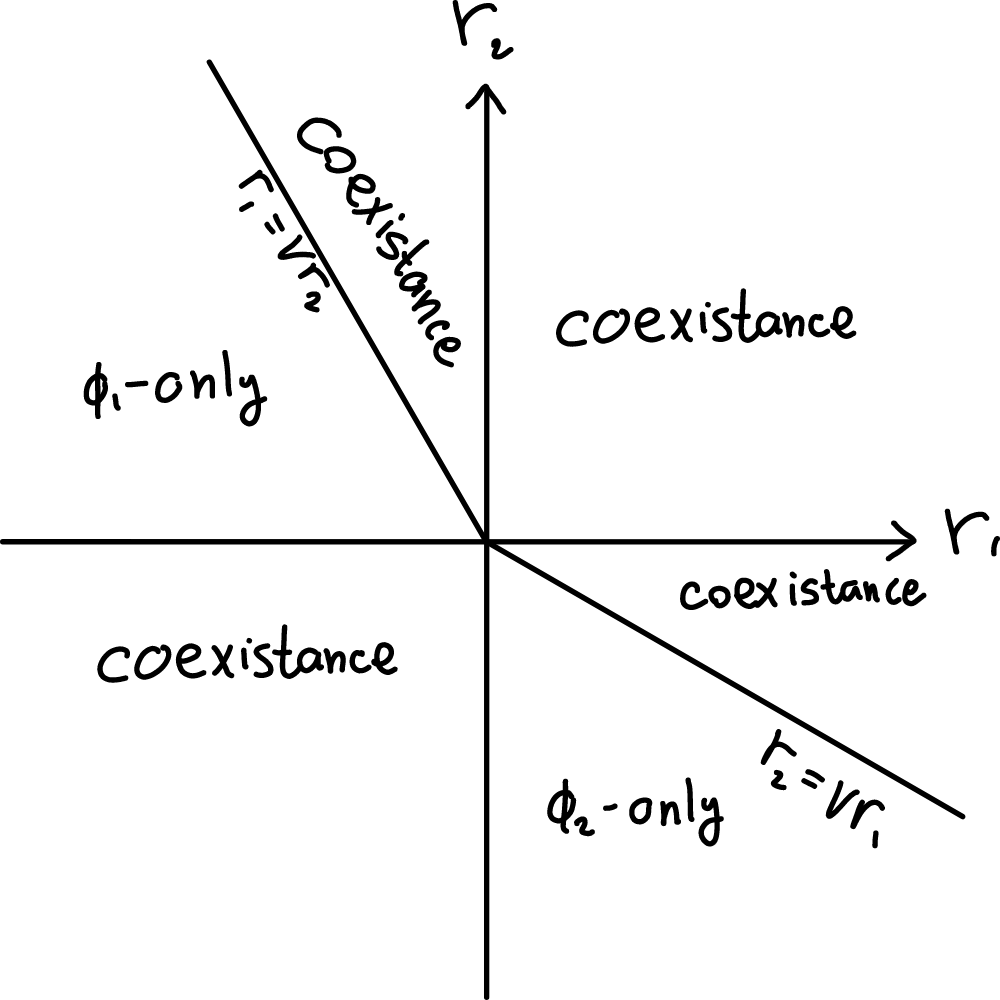
\includegraphics[width=0.5\textwidth]{Notewise-Untitled 2025-12-30-20260209195718.png}
    \caption{The phase diagram for $v < 0$}
\end{figure}
\newline
Now let us discuss the $v > 0$ case. Starting from both $r_1 > 0$ and $r_2 > 0$ both fields are in the disordered phase and we get the paramgnetic phase.
\newline
Next, let us look at $r_1 > 0$ and $r_2 < 0$. This time, $\phi_1$ requires $\phi_2^2 > -r_1/v$, which results at the opposite requirement from last time:
\begin{equation}
    r_2 < vr_1
\end{equation}
This means there is the same critical line, only in the opposite direciton: below the line both fields can coexist while above it only the independent field remains.
\newline
Lastly, let us look at $r_1 < 0$ and $r_2 < 0$. In this case both fields require the condition above, and we get:
\begin{equation}
    r_2 < vr_1 < v^2 r_2 \rightarrow v^2 < 1
\end{equation}
Where this time the direction flipped because we divided by $r_2 < 0$. This condition is again always met, and we get a coexsitance phase. The phase diagram for $v > 0$ can be seen in figure 3.
\begin{figure}[h]
    \label{fig:pos_v}
    \centering
    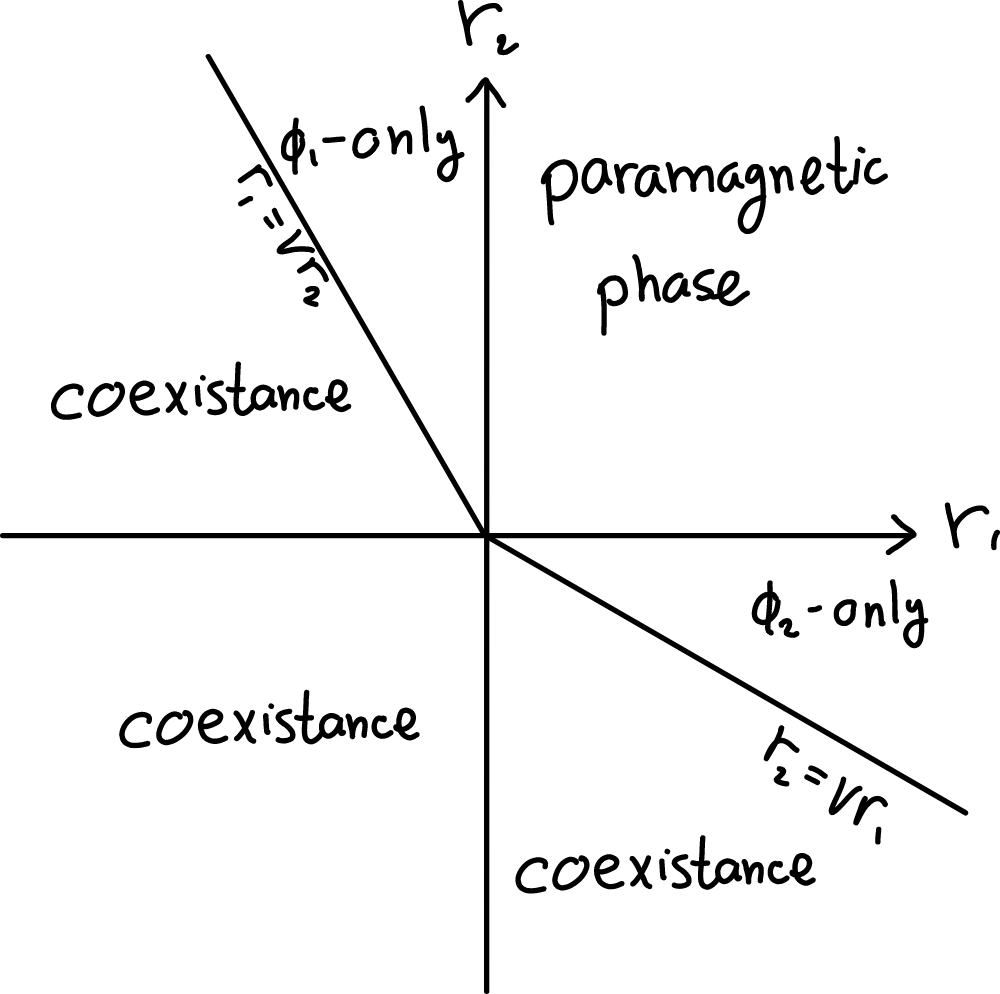
\includegraphics[width=0.5\textwidth]{Notewise-Untitled 2025-12-30-20260209195733.png}
    \caption{The phase diagram for $v > 0$}
\end{figure}
The major difference between the cooperative coupling $v < 0$ and the competitive coupling $v > 0$. In the cooperative coupling, almost the entire map is in coexistance. This results from the interaction canceling the paramagnetic phase completely. On the other hand, in competitive coupling, above the critical lines in the second and fourth quadrant, the two fields cannot coexist, and thus "compete".
\newline
Additinnally, from the formulas for $(\phi_1^2)_min, (\phi_2^2)_min$, we can find where the phase transition is first and second order. We can see that the fields become along the critical lines $r_1 = vr_2$ and $r_2 = vr_2$, making those a second order phase transition, while the other transitions, along the $r_1 = 0$ and $r_2 = 0$ lines are first order phase transitions.
\newline
Lastly, let us look at the special case $v = 1$. In this case, the free energy can be written as:
\begin{equation}
\begin{gathered}
    F = const +
    \frac{r_1}{2}\phi_1^2 +
    \frac{r_2}{2}\phi_2^2 +
    \frac{1}{4}\phi_1^4 +
    \frac{1}{4}\phi_2^4 +
    \frac{1}{2}\phi_1^2\phi_2^2 = \\ =
    const +
    \frac{r_1 + r_2}{2}(\phi_1^2 + \phi_2^2) +
    \frac{1}{4}(\phi_1^2 + \phi_1^2)^2
\end{gathered}
\end{equation}
Defining $\vec{\phi} = (\phi_1, \phi_2)$ and $r = r_1 + r_2$ gives:
\begin{equation}
    F = const + \frac{r}{2}\vec{\phi}^2 + \frac{1}{4}\vec{\phi}^4
\end{equation}
This is exactly the Landau theory for the XY model. In the same way, for $v = -1$, we can define $\psi = \phi_1 + i \phi_2$ which will give:
\begin{equation}
    F = const + \frac{r}{2}|\psi|^2 + \frac{1}{4}|\psi|^4
\end{equation} 
This is exactly the Landau theory for a complex valued field with phase symmetry.
\section{RG flow in the $\epsilon$-expansion on the same model}
Let us look at the same model using the $\epsilon$-expansion framework. Assuming they follow the relations:
\begin{equation}
    \frac{dv}{dl} = \epsilon v - 2v(u_1 + u_2)
    \qquad
    \frac{du_1}{dl} = \epsilon u_1 - (v^2 + u_1^2)
    \qquad
    \frac{du_2}{dl} = \epsilon u_2 - (v^2 + u_2^2)
\end{equation}
where l is the log of the length scale and $\epsilon = 4 - d$.
\subsection{Fixed points in useful subspaces}
Let us look first at the decoupled subspace $v = 0$. Plugging this into the equations gives (the first equation vanishes):
\begin{equation}
    \frac{du_1}{dl} = \epsilon u_1 - u_1^2
    \qquad
    \frac{du_2}{dl} = \epsilon u_2 - u_2^2
\end{equation}
This gives, in addition to the gaussian fixed point $(u_1, u_2) = (0,0)$, also the fixed points $(0,\epsilon), (\epsilon, 0), (\epsilon,\epsilon)$.
\newline
Now let us look at the symmetric subspace $u_1 = u_2 = u$. In this case we get (the second and third equations conincide):
\begin{equation}
    \frac{dv}{dl} = \epsilon v - 4uv
    \qquad
    \frac{du}{dl} = \epsilon u - (v^2 + u)
\end{equation}
Solving for $v$ first, we get $v = 0$ and $v = \frac{\epsilon}{4u}$ for $u \ne 0$:
We are looking for fixed points iwth $v \ne 0$, so let us plug the second value into the equation for $u$:
\begin{equation}
    (1-\epsilon)u - \frac{\epsilon^2}{16u^2} = 0
\end{equation}
This gives:
\begin{equation}
    u = \left(\frac{\epsilon^2}{16(1-\epsilon)}\right)^{1/3}
\end{equation}
But since this vanishes to first order:
\begin{equation}
    \frac{\epsilon^2}{1-\epsilon} = 
    \frac{1}{1-\epsilon} - \frac{1 - \epsilon^2}{1-\epsilon} = 
    \frac{1}{1-\epsilon} - (1 + \epsilon) \approx
    1 + \epsilon - (1 + \epsilon) = 0 
\end{equation}
We can conclude that there are no fixed points in this subspace.
\subsection{Relevance of $v$ at the decoupled fixed point}
Let us now linearize the v-flow around the fixed points of the decoupled space $v = 0$:
\begin{equation}
\begin{gathered}
    \frac{d\delta v}{dl} = \epsilon \delta v - 2\delta v(u_1 + u_2)
    \\
    \frac{d\delta u_1}{dl} = \epsilon \delta u_1 - (u_1^2 + 2u_1\delta u_1)
    \\
    \frac{d\delta u_2}{dl} = \epsilon \delta u_2 - (u_2^2 + 2u_2 \delta u_2)
\end{gathered}
\end{equation}
Starting from $(u_1, u_2) = (0, 0)$, we get:
\begin{equation}
\begin{gathered}
    \frac{d\delta v}{dl} = \epsilon \delta v
    \qquad
    \frac{d\delta u_1}{dl} = \epsilon \delta u_1
    \qquad
    \frac{d\delta u_2}{dl} = \epsilon \delta u_2
\end{gathered}
\end{equation}
Where the flow matrix is just the unit matrix multiplied by $\epsilon$. This means all of the eigenvalues are positive which makes this an unstable fixed point, with all directions relevant. Next, let us look at the point $(\epsilon, 0)$:
\begin{equation}
    \frac{d\delta v}{dl} = - \epsilon\delta v
    \qquad
    \frac{d\delta u_1}{dl} = - \epsilon\delta u_1
    \qquad
    \frac{d\delta u_2}{dl} = \epsilon \delta u_2
\end{equation}
This time, two directions are negative, making this an unstable point, with only one relevant direction.
Finally, let us trun to $(\epsilon, \epsilon)$ (the point $(0,\epsilon)$ is identical to the previous point):
\begin{equation}
    \frac{d\delta v}{dl} = -3\delta v
    \qquad
    \frac{d\delta u_1}{dl} = -\epsilon \delta u_1
    \qquad
    \frac{d\delta u_2}{dl} = -\epsilon \delta u_2
\end{equation}
This time all three eigenvalue are negative, making all three directions irrelevant.
\newline
In general, it seems that a perturbation $\delta v$ in the coupling between the order parameters will not change the theory.
\subsection{RG Flow}
I didn't have time to finish this (I know, eight hours is a lot), so just in short:
Adding the fluctuations to the symmetric subspace should not create fixed points since in the gaussian limit these fluctuations terms vanish, which is where the fixed points in this space is.
\end{document}